\documentclass[a4paper]{article}
\usepackage[utf8]{inputenc}
\usepackage[spanish, es-tabla]{babel}

\usepackage[a4paper, footnotesep = 1cm, width=18cm, left=2cm, top=2.5cm, height=25cm, textwidth=18cm, textheight=25cm]{geometry}
%\geometry{showframe}

\usepackage{tikz}
\usepackage{amsmath}
\usepackage{amsfonts}
\usepackage{amssymb}
\usepackage{float}
\usepackage{graphicx}
\usepackage{caption}
\usepackage{subcaption}
\usepackage{multicol}
\usepackage{multirow}
\setlength{\doublerulesep}{\arrayrulewidth}
\usepackage{xcolor}

\usepackage{hyperref}
\hypersetup{
    colorlinks=true,
    linkcolor=blue,
    filecolor=magenta,      
    urlcolor=blue,
    citecolor=blue,    
}

\newcommand{\quotes}[1]{``#1''}
\usepackage{array}
\newcolumntype{C}[1]{>{\centering\let\newline\\\arraybackslash\hspace{0pt}}m{#1}}
\usepackage[american]{circuitikz}
\usepackage{fancyhdr}
\usepackage{units} 

\pagestyle{fancy}
\fancyhf{}
\lhead{22.13 Electrónica III}
\rhead{Mechoulam, Lambertucci, Martorell, Londero}
\rfoot{\center \thepage}

\begin{document}
\subsection{Introducción}

En esta sección se procedió a realizar el análisis de dos compuertas lógicas de distintas tecnologías, las cuales que consisten en una compuerta AND de tecnología TTL y una compuerta OR CMOS, conectadas de la siguiente forma
\begin{figure}[H]
\begin{center}
\begin{circuitikz}
	\node [american and port](A){TTL};
	\draw (A.out) to[short, -o] ++(1,0) node[label=right:$Port$](){};
	\draw (A.in 1) to[short, -o] ++(-1,0) node[label=left:$V_{CC}$](){};
	\draw (A.in 2) to[short, -*] ++(-0.5,0);
	
	\draw (A) to[open] ++(0,-2) node[american or port](O){\footnotesize{MOS}};
	\draw (O.out) to[short, -o] ++(1,0) node[label=right:$Port$](){};
	\draw (O.in 2) to[short] ++(-1,0) node[ground](){};
	\draw (O.in 1) to[short, -*] ++(-0.5,0);
\end{circuitikz}
\caption{Circuitos en vacío.}
\label{fig:circ-vacio}
\end{center}
\end{figure}

\subsection{Análisis compuerta AND Open Gate}

Para realizar este análisis se utilizó una de las 4 compuertas que brinda el integrado \href{http://www.ti.com/lit/ds/symlink/sn74s08.pdf}{SN74S08}. Como es una compuerta AND, y una de sus entradas ya esta conectada a $V_{CC}$, la señal de salida dependerá solo del valor que tenga la señal en esa sola entrada. Ahora, dejando al vacío esa entrada, se puede observar una tensión continua de valor aproximado $1.45 \ V$, que corresponde al rango de valores que la compuerta considera como indeterminados, obteniéndose así a la salida un 1 lógico. Esto ocurre debido a que se esta dejando al vacío el emisor del transistor al que le corresponde esa entrada, por lo tanto dicho transistor se encuentra al corte, lo que hace que a la salida siempre se vea dicho valor. A su vez se procedio a tocar con la mano un cable que hacia contacto con la entrada de la compuerta que se encuentra al vacio y se obtuvo lo siguiente:

\begin{figure}[H]
    \centering
    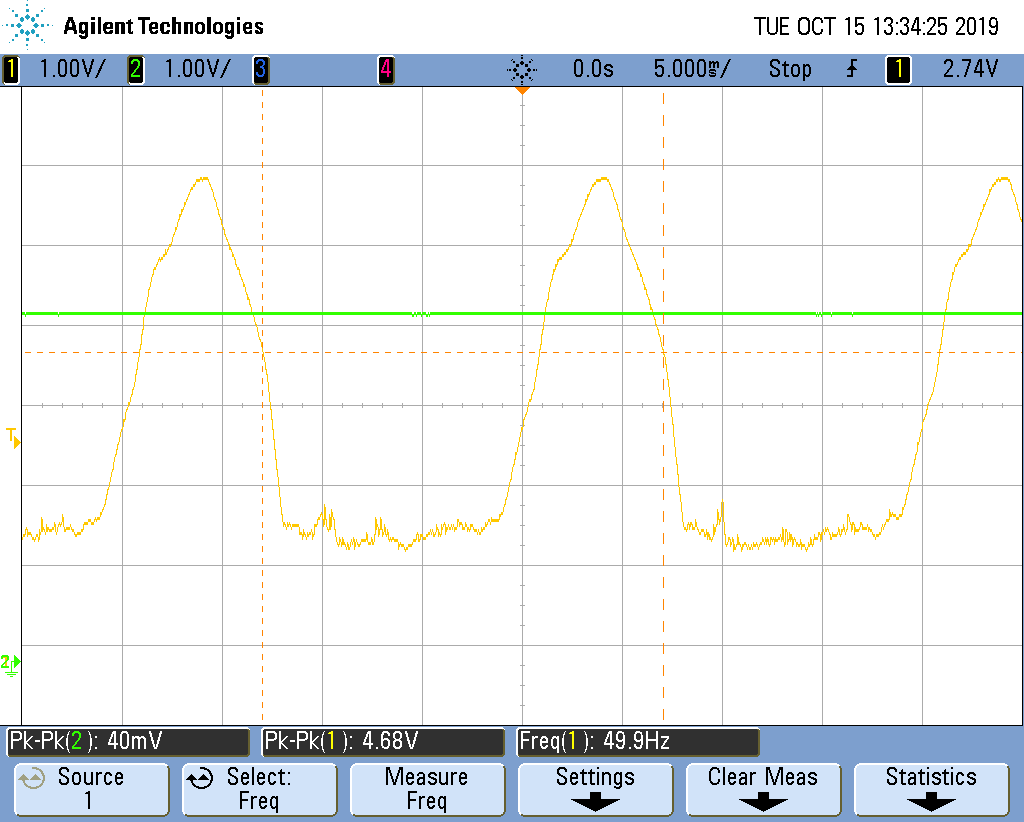
\includegraphics[scale=0.30]{/ImagenesEjercicio5/ari_e4.png}
    \caption{Señal a la salida de la AND con una entrada en vacio otra a VCC}
\end{figure}

Analizando la figura anterior se puede notar la mayor resistencia al ruido que presenta la compuerta ya que a pesar de que a la entrada se presenta una oscilación de frecuencia $f=50 Hz$ la salida se mantiene e un valor constante.



\subsection{Análisis compuerta OR Open Gate}

De forma análoga al caso anterior, se utilizó una de las compuertas lógicas que brinda el integrado \href{http://www.ti.com/lit/ds/symlink/cd4071b.pdf}{CD4071}, pero en este caso, se conecto uno de sus pines de entrada a $GND$, dejando el otro abierto. Es así que el valor que se ve a la salida depende únicamente del valor de la entrada que se dejó abierta. Como esta compuerta es de tecnología MOS, conectándose a su entrada el GATE de un transistor de este mismo tipo, y debido a la gran impedancia de entrada que poseen, actúan como antena, lo que las hace mas susceptibles a cualquier señal de ruido que se encuentre presente. Teóricamente, si dicha señal de ruido llega a poseer una tensión lo suficientemente alta como para superar la $V_{TH}$ del transistor, este se activa y produce una oscilación a la salida de la compuerta. Se realizarón distintas pruebas para poder ver este fenómeno, cuando se dejaba la entrada en vacio se llegaba a apreciar una cierta cantidad de ruido pero no la suficiente para obtener alguna señal a la salida por lo tanto se tocó con la mano un cable que estaba en contacto con dicha entrada y con esto se pudo apreciar una oscilación a la salida que se puede observar en la siguiente figura:


\begin{figure}[H]
    \centering
    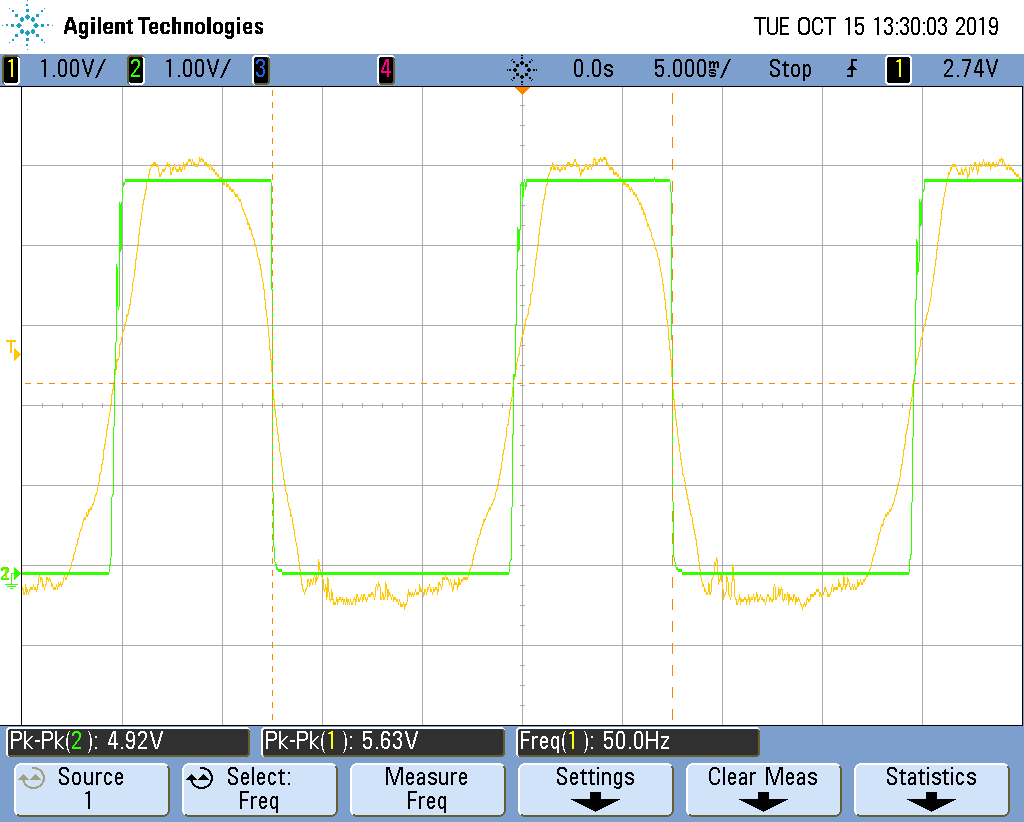
\includegraphics[scale=0.30]{/ImagenesEjercicio5/ari_e3.png}
    \caption{Señal a la salida de la OR con una entrada en vacio otra a ground}
    
\end{figure}

Como se puede observar de la figura anterior la salida oscila a una frecuencia de $50 Hz$ que corresponden a la frecuencia del ruido de linea.


Luego, se conecto los circuitos de la siguienta manera:
\begin{figure}[H]
\begin{center}
\begin{circuitikz}
	\node [american and port](A){};
	\draw (A.in 1) to[short, -o] ++(-1,0) node[label=left:$V_{CC}$](){};
	\draw (A.in 2) to[short, -o] ++(-1,0) node[label=left:$Input$](){};
	
	\draw (A.out) |- ++(0,-1) node[american or port, anchor=in 1](O){};
	\draw (O.out) to[short, -o] ++(1,0) node[label=right:$Port$](){};
	\draw (O.in 2) to[short] ++(-0.5,0) node[ground](){};
\end{circuitikz}
\caption{Conexión AND a la entrada de la OR.}
\label{fig:circ-andor}
\end{center}
\end{figure}

La salida de este, por lo analizado en los anteriormente, solo depende de la señal de entrada que se utiliza. Analizando las hojas de datos de ambos integrados y utilizando una alimentación $V_{DD}= 4.5 \ V$, se obtiene que la tensión mínima de la salida en estado alto es $V_{OH}=2.5 \ V$, la cual cae en el rango de valores indeterminados para la OR, siendo esta $V_{IL}= 3.15 \ V$ en el peor de los casos. Es así que se puede ocasionar que, a pesar de que la salida de la AND sea HIGH, en la salida total del circuito se vea un 0 lógico.

\subsection{Solución al problema}

Una solución al problema mencionado anteriormente se basa en utilizar un circuito llamado Level Shifter, el cual se puede fabricar utilizando un transistor PNP y un par de resistencias. Este circuito toma la salida de la primer compuerta y, en el caso de que está sea HIGH, lleva dicho valor a un nivel de tensión más alto para que así la compuerta siguiente pueda tomar correctamente el valor que debe recibir. Dicha solución se implemento al circuito anterior y se pudo solucionar el problema.
\begin{figure}[H]
\begin{center}
\begin{circuitikz}
	\node [pnp](pnp){};
	\draw (pnp.E) to[R, -o] ++(0,2) node[label=left:$V_{CC}$](){};
	\draw (pnp.C) to[short] ++(0,-0.5) node[ground](){};
	\draw (pnp.B) to[R, -o] ++(-2,0) node[label=left:$Input$](){};
\end{circuitikz}
\caption{Implementación del level shifter.}
\label{fig:levelshifter}
\end{center}
\end{figure}

\end{document}